The PLC (Programmable Logic Controller) is the central control unit responsible for executing the palletizing process in a predefined sequence. It receives inputs from various sensors and controls the UR20 arm, conveyor belt, and gripper systems. The PLC is programmed to execute a routine to efficiently manage the automation cycle.
\subsection{Layer Hardware}
The PLC layer utilizes the same hardware as the subsystem which is isted below.

\subsection{Layer Operating System}
The PLC utilizes a Real-Time Operating System to ensure timely and deterministic control of hardware components.

\subsection{Box Placement Routine}

The Box Placement Routine governs the entire palletizing sequence, ensuring efficient box handling. It takes input from the safety and photo eye sensor, processes the data, and outputs commands to control the conveyor belt, vacuum gripper, and UR20 robot arm.

\begin{figure}[h!]
	\centering
 	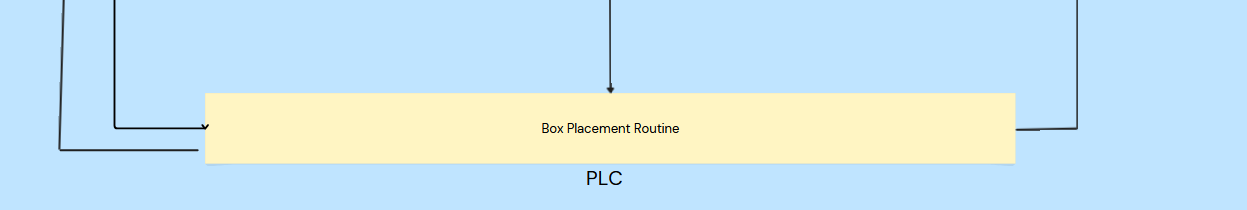
\includegraphics[width=0.60\textwidth]{images/plc.png}
 \caption{Box Placement Routine diagram}
\end{figure}

\subsubsection{Subsystem Hardware}
The Box Placement Routine subsystem utilizes the hardware from each layer as follows:
    \begin{itemize}
        \item Photo Eye Sensor: Provides input to detect boxes on the conveyor belt
        \item Safety Laser Scanner: Provides input to ensure safe operation
        \item Conveyor Belt Motor: Controlled by the PLC to turn ON/OFF
        \item Vacuum Gripper: Controlled by the PLC to pick and release boxes.
        \item UR20 Robot Arm: Moves to predefined positions for picking and placing boxes
    \end{itemize}

\subsubsection{Subsystem Operating System}
PolyScope is the software included on the 3PE Teach Pendant, utilized in setting the predefined arm movements.

\subsubsection{Subsystem Software Dependencies}
URX Python library

\subsubsection{Subsystem Programming Languages}
URSCript and Python are used to control the PLC.

\subsubsection{Subsystem Data Structures}
\begin{itemize}
    \item Sensor Data Packets:
        \begin{itemize}
            \item Photo Eye Sensor: Binary Bit (box detected or not)
            \item Safety Scanner: Binary Bit (object in range or not)
        \end{itemize}
    \item Robot Position Data: Predefined coordinates and angles for picking and placing boxes.
    \item Conveyor Belt Status: Binary Bit (ON/OFF)
    \item Vacuum Gripper Status: Binary Bit (Activated/Deactivated)
\end{itemize}

\subsubsection{Subsystem Data Processing}
The Box Placement Routine follows a state-driven algorithm, executing the following logic:
\begin{enumerate}
    \item IF Phot Eye Sensor detects a box --> STOP conveyor belt.
    \item IF safety laser scanner detects object in range of robot --> Adjust UR20 movement speed/ Halt all movement
    \item Activate vacuum gripper and move UR20 to box position
    \item Move to predefined pallet position
    \item Release vacuum gripper and return UR20 to standby position
    \item Turn conveyor belt on
    \item Repeat until palletizing sequence is complete
\end{enumerate}